\section{Teil}

%-------------------------------------------------------------------------------------------
\subsection{Wie kann Komplexität von Systemen charakterisiert werden?}
\textbf{Komplexität} beschreibt, dass das Verhalten eines Modells schwierig zu beschreiben ist, obwohl ausreichend Information über seine Komponenten
 und deren Verflechtungen vorliegen.Was als komplex gilt kommt immer auf die Sichtweise drauf an. $\rightarrow$ Schwer es allgemein zu definieren.
\\

Ein \textbf{komplexes System} ist ein System mit einer großen Zahl and Komponenten und Verknüpfungen, Interaktionen oder Abhängigkeiten, 
welches schwierig beschreibbar, planbar oder steuerbar ist.

\begin{figure}[H]
	\centering
	\includegraphics[width=0.6\linewidth]{Bilder/Teil1_Komplexität.png}
	\caption{Swimlane Diagramm}
\end{figure}

% subsection
%-------------------------------------------------------------------------------------------
\subsection{Nennen Sie externe und interne Komplexitätstreiber!}
	

\begin{table}[h!]
	\centering
	\begin{tabular}{|p{7cm}|p{7cm}|}
		\hline
		\multicolumn{1}{|c|}{\textbf{Externe}} & \multicolumn{1}{c|}{\textbf{Interne}} \\ \hline
		Heterogene Märkte & Aufwendiges Produktkonzept \\ \hline
		Individuelle Kundenbedürfnisse & Hohe Komponentenvielfalt \\ \hline
		Erforderliche Variantenvielfalt & Komplexer Entwicklungsprozess \\ \hline
		Wettbewerb und Gesetzte & Komplexe Fertigung \\ \hline
		Preisdruck & Viele Zulieferer und Projektbeteiligte \\ \hline
	\end{tabular}
	\caption{Vergleich von externen und internen Faktoren}
	\label{tab:extern-intern}
\end{table}
\textbf{Die kann die internen Komplexitätstreiber selber vielleicht beeinflussen die externen nicht!}

% subsection
%-------------------------------------------------------------------------------------------
\subsection{Was versteht man unter Cyber-Physikalischen Systemen}

\begin{itemize}
	\item \textbf{Eine Integration von Computern und physischen Prozessen:}
	\\Physische Prozesse werden durch eingebettete Computer und Netzwerke überwacht, geregelt und gesteuert.
	\item \textbf{Gegenseitige Rückkopplung:} 
	\\Computer und physische Prozesse beeinflussen sich gegenseitig. (Wechselwirkung)
	\item \textbf{Beispiele:} 
	\\Autonome Fahrzeuge, Smartwatch, Produktionsanlagen.
\end{itemize}

% subsection
%-------------------------------------------------------------------------------------------
\subsection{Was versteht man unter Internet of Things}
\begin{itemize}
	\item \textbf{Ein globales Netzwerk von physischen und virtuellen Objekten:} 
	\\Diese Objekte kommunizieren und arbeiten zusammen.
	\item \textbf{Technologie zur Unterstützung des Menschen:}
	\\Ermöglicht Interaktion zwischen Mensch und vernetzten Systemen sowie zwischen den Systemen selbst.
	\item \textbf{Beispiele:} 
	\\Kühlschränke mit automatischer Nachbestellung. Hat sich besonders bei Supermärkten durchgesetzt
\end{itemize}


% subsection
%-------------------------------------------------------------------------------------------
\subsection{Was versteht man unter Systems of Systems?}
Ein Systems of Systems (SoS) ist:
\begin{itemize}
	\item \textbf{Ein Verbund autonomer Systeme:} 
	\\Diese Systeme arbeiten zusammen, um ein neues, komplexeres System mit zusätzlicher Funktionalität zu schaffen.
	
	\item \textbf{Charakteristische Merkmale:}
	\begin{itemize}
		\item \textbf{Operative Unabhängigkeit der Subsysteme:} Jedes Subsystem arbeitet unabhängig.
		\item \textbf{Unabhängige Verwaltung der einzelnen Systeme:} Die Systeme werden eigenständig verwaltet.
		\item \textbf{Evolutionäre Entwicklung:} Ständige Weiterentwicklung und Anpassung der Systeme/Komponenten. (ohne das das gesamt System zusammenbricht)
		\item \textbf{Emergentes Verhalten:} Ausfall von einem Teil führt nicht zum Ausfall des gesamten Systems.
		\item \textbf{Geografische Verteilung der Systeme:} Die Systeme können an verschiedenen geografischen Orten verteilt sein.
	\end{itemize}
\end{itemize}


% subsection
%-------------------------------------------------------------------------------------------
\subsection{Was ist ein Produkt-Service-System (PSS)? }
Ist ein \textbf{Leistungsangebot} mit signifikanten \textbf{Anteilen an Sachgütern als auch Dienstleistungen}. Dienstleistungen sind integraler Bestandteil des PSS. 

Z.B. Carsharing, Leasing

% subsection
%-------------------------------------------------------------------------------------------
\subsection{Welche Klassen von Produkt-Service-Systemen gibt es?}
Einteilung in 3 Teile:
\begin{itemize}
    \item \textbf{Reines Produkt}
        \begin{itemize}
            \item Produkt im Besitz des Kunden.
            \item Kunde selber verantwortlich.
            \item z.B. Kauf Waschmaschine, Auto
        \end{itemize}
    \item \textbf{Reiner Service}
        \begin{itemize}
            \item Reine Dienstleistung.
            \item Produkt nicht im Besitz des Kunden.
            \item z.B. Waschsalon, Beratung
        \end{itemize}

    \item \textbf{Produkt Service Systeme:}
    
    \begin{itemize}
    	\item \textbf{Produktorientiert:}
    	\begin{itemize}
    		\item Klassischer Verkauf im Vordergrund.
    		\item Produktbezogen, Beratung (Auto + Einschulung oder Wartung)
    	\end{itemize}
    	
    	\item \textbf{Nutzungsorientiert:}
    	\begin{itemize}
    		\item Nutzung des Produktes im Vordergrund.
    		\item Produkt im Besitz des Anbieters.
    		\item z.B. Leasing, Mieten, Pooling
    	\end{itemize}
    	
    	\item \textbf{Ergebnisorientiert:}
        \begin{itemize}
        	\item Ergebnis steht im Vordergrund
			\item Übereinkunft zwischen Anbieter und Kunde über zu erreichendes Ziel.
			\item Die Wahl des Produktes und des Vorgehens obliegt dem Anbieter.
			\item Honorar nach Ergebnis
		\end{itemize}
    	
    \end{itemize}
        
\end{itemize}

% subsection
%-------------------------------------------------------------------------------------------
\subsection{Aus welchen Bestandteilen besteht ein System?}

\begin{figure}[H]
	\centering
	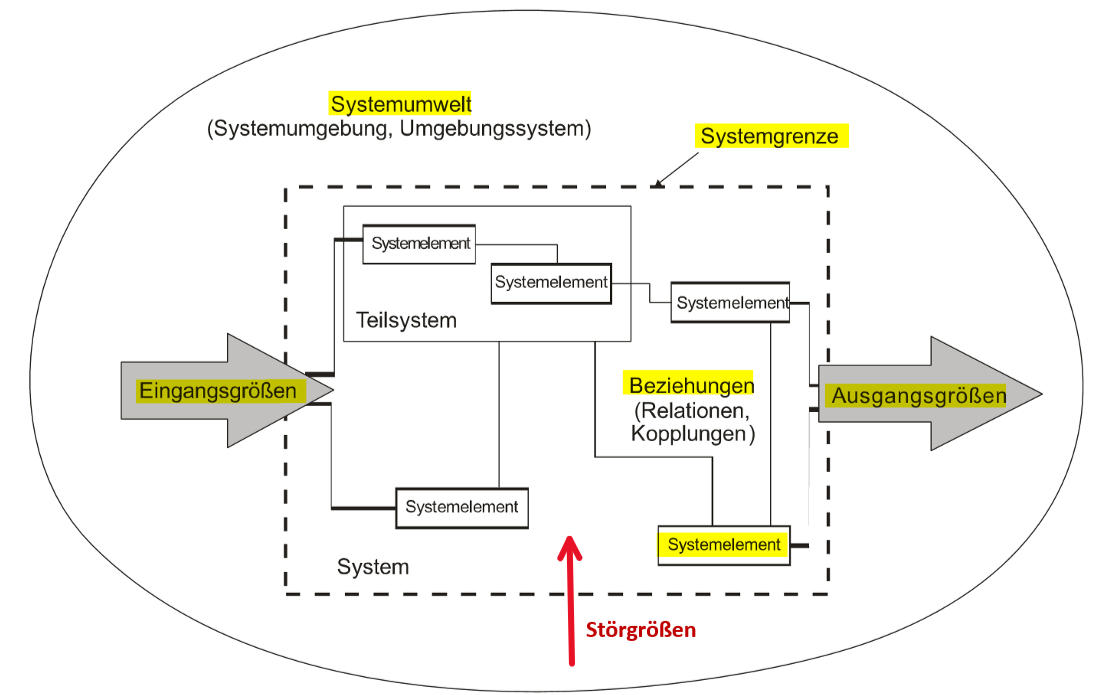
\includegraphics[width=0.7\linewidth]{Bilder/Teil1_zentraleDarstellungSystem.png}
	\caption{Swimlane Diagramm}
\end{figure}

\begin{itemize}
    \item \textbf{Systemumwelt}
    \begin{itemize}
        \item Alles, was nicht in das System einbezogen ist (abgetrennt an Systemgrenze).
    \end{itemize}
    
    \item \textbf{Stoff-, Energie-, Informationsfluss}
    \begin{itemize}
        \item Art und Weise der Interaktion mit Systemumwelt.
        \item Systemgrenze so wählen, dass Kopplung zur Umgebung sehr viel schwächer als Kopplung im Inneren ist.
    \end{itemize}
    
    \item \textbf{Eingang}
    \begin{itemize}
        \item Stellt Relation der Umwelt zum System dar.
        \item Vom Verhalten des Systems nicht beeinflusst.
        \item \textbf{Stellgrößen}: gezielte Veränderung des Eingangs.
        \item \textbf{Störgrößen}: unkontrollierte Veränderung des Eingangs (z.B. Rauschen).
    \end{itemize}
    
    \item \textbf{Ausgang}
    \begin{itemize}
        \item Stellt Relation vom System zur Umgebung dar (z.B. Messgröße).
    \end{itemize}
    
    \item \textbf{Teilsystem}
    \begin{itemize}
        \item Element eines Systems, welches weitere Elemente enthält (enthält eigenes System - Subsystem).
    \end{itemize}
    
        \item \textbf{Störgrößen}
    \begin{itemize}
    	\item Nicht gewünschte Eingangsgrößen (Bsp. Rauschen)
    \end{itemize}
    
\end{itemize}

% subsection
%-------------------------------------------------------------------------------------------
\subsection{Begriffe wofür Systems Engineering steht!}
\begin{itemize}[itemsep=0pt, topsep=10pt]
    \item Interdisziplinär
    \item Früh (in Entwicklungsprozess)
    \item Dokumentieren (Anforderungen)
    \item Gesamtheitlich (auf System Bezogen)
    \item Wirtschaftlich (Bedürfnisse des Kunden)
    \item Technisch
\end{itemize}

% subsection
%-------------------------------------------------------------------------------------------
\subsection{Was bedeutet SADT + Beispiel.}
\textbf{SADT = Structured Analysis and Design Technique}

Beschreibt Aktivitäten und Informationsflüsse. z.B. Bauteilbearbeitung

\begin{figure}[H]
    \centering
    \begin{minipage}[t]{0.45\textwidth}  % 't' sorgt dafür, dass die minipage an der Oberkante ausgerichtet ist
        \centering
        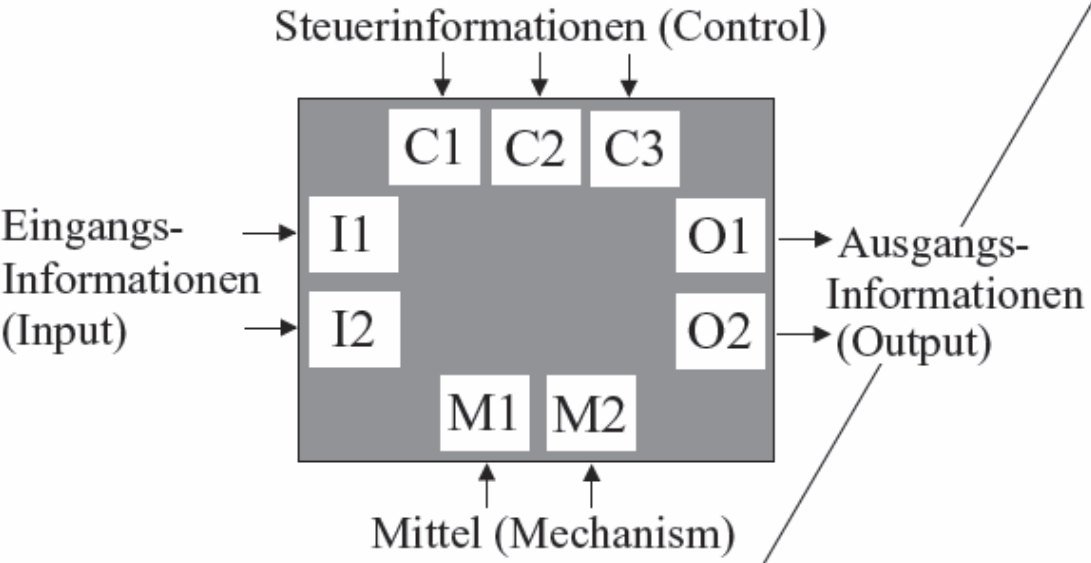
\includegraphics[width=\linewidth]{Bilder/Teil1_SADT_Allgemein.png} % Bild 1
        \caption{SADT Allgemein}
    \end{minipage} \hfill
    \begin{minipage}[t]{0.45\textwidth}  % 't' sorgt für gleiche Ausrichtung der Unterschriften
        \centering
        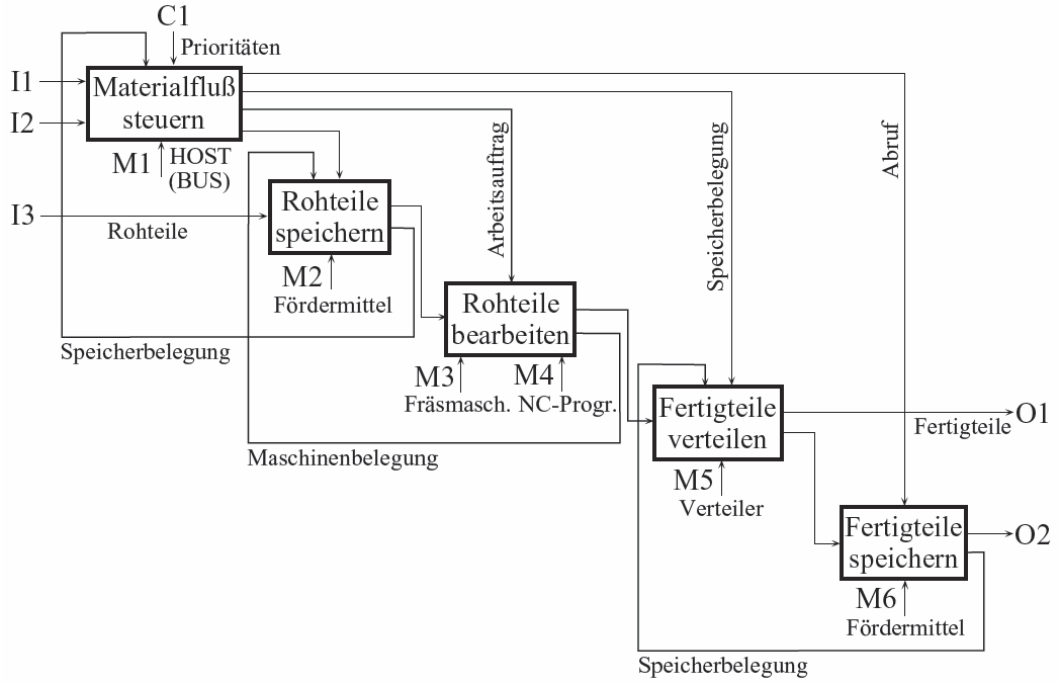
\includegraphics[width=\linewidth]{Bilder/Teil1_SADT_Beispiel.png} % Bild 2
        \caption{SADT Praxisbeispiel}
    \end{minipage}
    %\caption{Structured Analysis and Design Technique - SADT}
\end{figure}




% subsection
%-------------------------------------------------------------------------------------------
\subsection{Was sind Swimlane-Diagramme + Beispiel}
Sind eine Art von \textbf{Flussdiagrammen}, welche zeigen wer in einem Prozess zuständig ist.

\textbf{Verantwortungsbereiche = Swimlanes}

\begin{figure}[H]
    \centering
    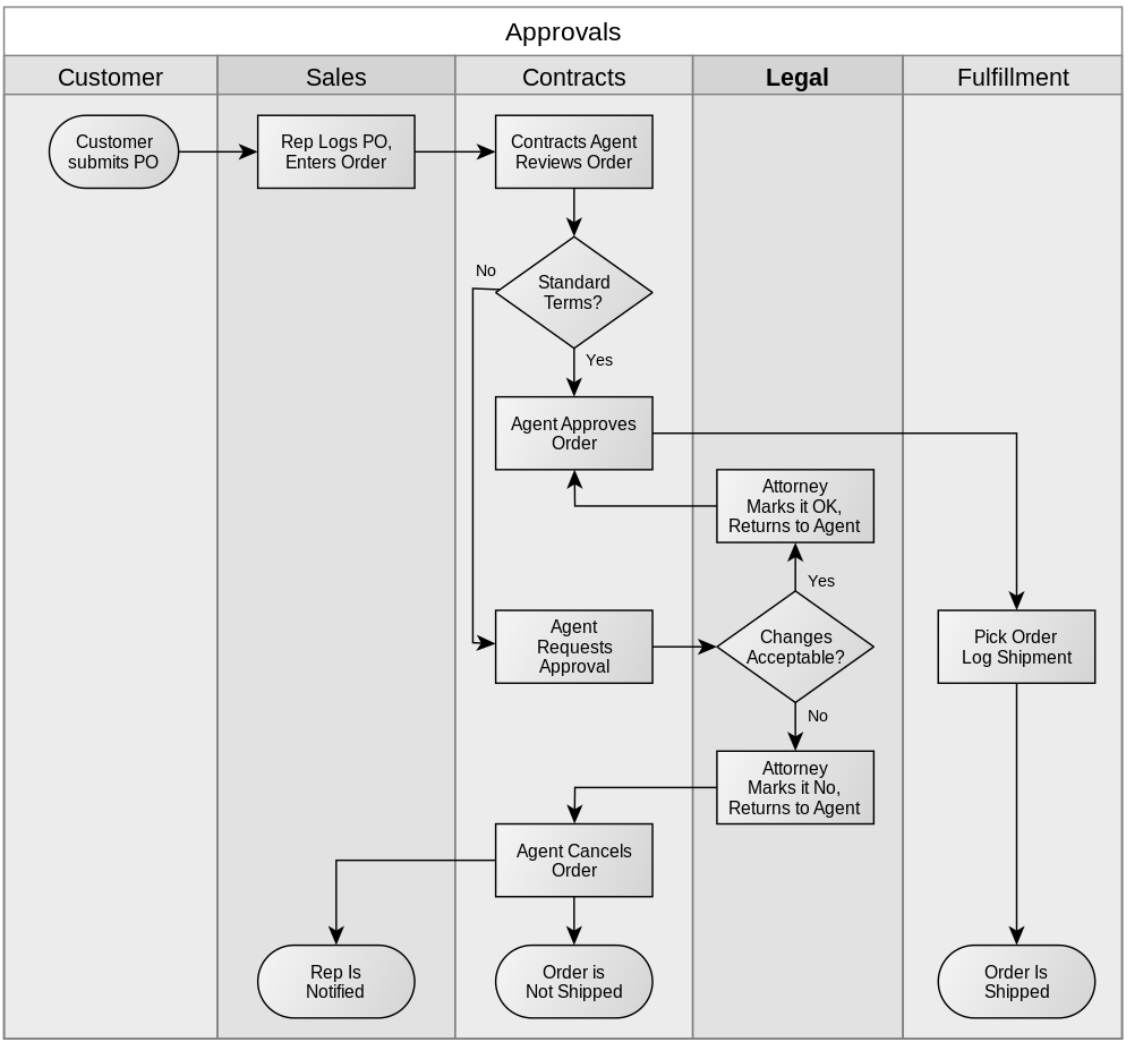
\includegraphics[width=0.7\linewidth]{Bilder/Teil1_SwimlaneDiagramm.png}
    \caption{Swimlane Diagramm}
\end{figure}

% subsection
%-------------------------------------------------------------------------------------------
\subsection{Vier Grundregeln des Agilen Manifests}

\textbf{Grundlagen - Theoretisch}
\begin{itemize}
    \item Individuen und Interaktionen haben Vorrang zu Prozessen und Werkzeugen
    \item Funktionsfähige Produkte haben Vorrang zu ausgedehnter Dokumentation
    \item Zusammenarbeit mit Kunden hat Vorrang vor Vertragshandlungen
    \item Reagieren auf Änderungen hat Vorrang vor strikter Planverfolgung
\end{itemize}

\textbf{Grundlagen - Praxisbeispiele}
\begin{itemize}
    \item Arbeiten im Team
    \item Fokus auf technische Aufgabenstellung
    \item Denke an Kunden
    \item Flexibel für Änderungen
\end{itemize}

% subsection
%-------------------------------------------------------------------------------------------
\subsection{Bedeutung SCRUM + Rollen  }
\textbf{SCRUM = Vorgehensmodell der agilen Softwareentwicklung.}

Geht davon aus, dass Entwicklungen aufgrund ihrer Komplexität nicht im Vorraus detailliert planbar sind.

\textbf{Stärken:} überschaubares Rahmenwerk mit wenig Rollen, Artefakten und Ereignissen.

\textbf{Rollen}
\begin{itemize}
    \item Product Owner
    \begin{itemize}
        \item Für wirtschaftlichen Erfolg des Produktes verantwortlich.
        \item Vertritt Kundeninteressen. Sind aber nicht identisch.
    \end{itemize}
    
    \item Entwickler Team
    \begin{itemize}
        \item Keine hierarchischen Strukturen.
        \item Setzt Anforderungen von Product Owner um.
    \end{itemize}
    
    \item Scrum Master
    \begin{itemize}
        \item Moderiert alle Ereignisse und sorgt für störungsfreies Arbeiten.
        \item Kein Teammitglied und nicht weisungsbefugt.
        \item Stellt Einhaltung von Scrum-Regeln sicher.
    \end{itemize}
    
\end{itemize}
